\chapter{Method and Datasets}
\label{sec:method}
In this chapter, the specific neural network used to denoise \acrshort{ct} images will be introduced, some image comparison metrics will be given alongside a brief discussion of them, the used datasets will be described, and the method used to compile a given dataset into a suitable format for the neural network will be explained. 


\section{TomoGAN}
\label{sec:method:tomogan}
\todo[inline]{GAN where input is not random, but noisy image. U-net structure (encoder-decoder). Extract feature map of noisy image where noise is removed, and generate image from noiseless feature map. }
TomoGAN \cite{liu2020tomogan}


\section{Image Comparison Metrics}
\label{sec:method:metrics}
To properly quantify the performance of the denoising algorithm, some metrics must be defined. While there are some standards to doing this, not all methods perform equally well. 

\subsection{Mean Squared Error}
\label{sec:method:metrics:mse}
The most commonly used full-reference image quality metric is the \acrfull{mse}, as defined (as a loss function) in \cref{eq:lossmse}. While it provides some sense of similarity and is very easy to calculate and physically understand, a low (i.e. good) \acrshort{mse} does not necessarily correspond to a visual similarity and it is therefore not a good metric to compare visual similarities in images \cite{413502,477498}. Likewise, the \acrfull{psnr}, which is another very commonly used metric, does not correspond to visual similarity. The \acrshort{psnr} can be defined from the \acrshort{mse}, and is given as \cite{477498}
\begin{equation}
    \label{eq:psnr}
    \text{PSNR} = 10 \cdot \log_{10} \left( \frac{\text{MAX}_Y}{MSE^2} \right),
\end{equation}
where $\text{MAX}_Y$ is the maximal pixel value possible in the image (e.g. for an 8-bit image it is $2^8-1=255$), and $MSE$ is the \acrshort{mse} of the image. 

\subsection{Structural Similarity Index Measure}
The \acrfull{ssim} is a metric to measure similarity between images \cite{ssim}. It is a full-reference image quality assessment, meaning it compares a complete reference high-quality image to a full low-quality image\footnote{Other types of image quality assessments are either no-reference where there is no high-quality reference image to compare to, or reduced-reference where there is some partial information from a reference image to compare to (e.g. a set of extracted features)\cite{ssim}. }. 


The \acrshort{ssim} takes into account three metrics of the image: luminance, contrast, and structure. They are combined, giving the definition of \acrshort{ssim} as \cite{ssim}
\begin{equation}
    \label{eq:ssim}
    \text{SSIM}\left(x,y\right) = \frac{\left( 2\mu_x \mu_y + C_1 \right) \left( 2\sigma_{xy} + C_2 \right)}{\left( \mu_x^2 + \mu_y^2 + C_1 \right) \left( \sigma_x^2 + \sigma_y^2 + C_2 \right)},
\end{equation}
where $x$ and $y$ are the two images to compare, $\mu$ is the mean pixel value of an image, $\sigma$ is the standard deviation of the pixel values of an image, and $C_{\{1,2\}}$ are regularization constants. It is symmetric (i.e. $\text{SSIM}\left(x,y\right) = \text{SSIM}\left(y,x\right)$), bounded (i.e. $\text{SSIM}\left(x,y\right) \leq 1$), and has a unique maximum (i.e. $\text{SSIM}\left(x,y\right) = 1$ if and only if $x = y$) \cite{ssim}. A more robust analysis of the mathematical properties of the \acrshort{ssim} was performed in \cite{6059504}.

\missingfigure{TODO: Maybe add figure showing difference in MSE and SSIM performance, similar to fig. 2 in \cite{ssim}. }

\section{Datasets}
\label{sec:method:datasets}
A selection of different datasets have been used to train and test the TomoGAN network. Some of these have been collected from TomoBank \cite{TomoBank}, while others are collected in-house. This section will give a description of each used dataset. 

\subsection{TomoBank}
TomoBank is an x-ray tomography data bank providing experimental and simulated datasets with the aim to foster collaboration among computational scientists, beamline scientists, and experimentalists \cite{TomoBank}. It provides several types of datasets imaging different samples. Some of these datasets have been used in this thesis.

\todo[inline]{Paragraph about tomo\_00058 linking it to the table. }

\begin{table}[htbp]
    \centering
    \caption[Dataset information tomo\_00058]{Overview of technical information of the tomo\_00058 dataset. A more complete overview is available from \cite{datasetglassspheres}. }
    \label{tab:tomo00058}
    \begin{tabular}{ll}
    \hline
    Instrument & APS 2-BM-A fast tomo \\
    Scan Range & 180 degree \\
    Number of Projections & 1500 \\
    Sample Detector Distance & \SI{60}{\milli \meter} \\
    Pixel size & \SI{0.65}{\micro \meter} \\
    Detector Dimension x & 2560 \\
    Detector Dimension y & 2160 \\
    \hline
    \end{tabular}
\end{table}

% \cite{datasetshale}. 
All datasets used from TomoBank were reconstructed using \acrshort{fbp} from the TomoPy library \cite{tomopy}. 


\subsection{In-house}
\todo[inline]{ASM\_ID16B\_phaseContrast\_Shale\_2018}
\todo[inline]{Kim-Roberts dataset}

\section{Compiling a Dataset for Training}
\label{sec:method:compilingdataset}
In this section, an explanation of how to compile a set of images into a suitable dataset for training the TomoGAN network will be given. % All these steps can be considered pre-processing. 

\todo[inline]{Flowchart not done yet, finish it. }

\begin{figure}[htbp]  
    \centering
    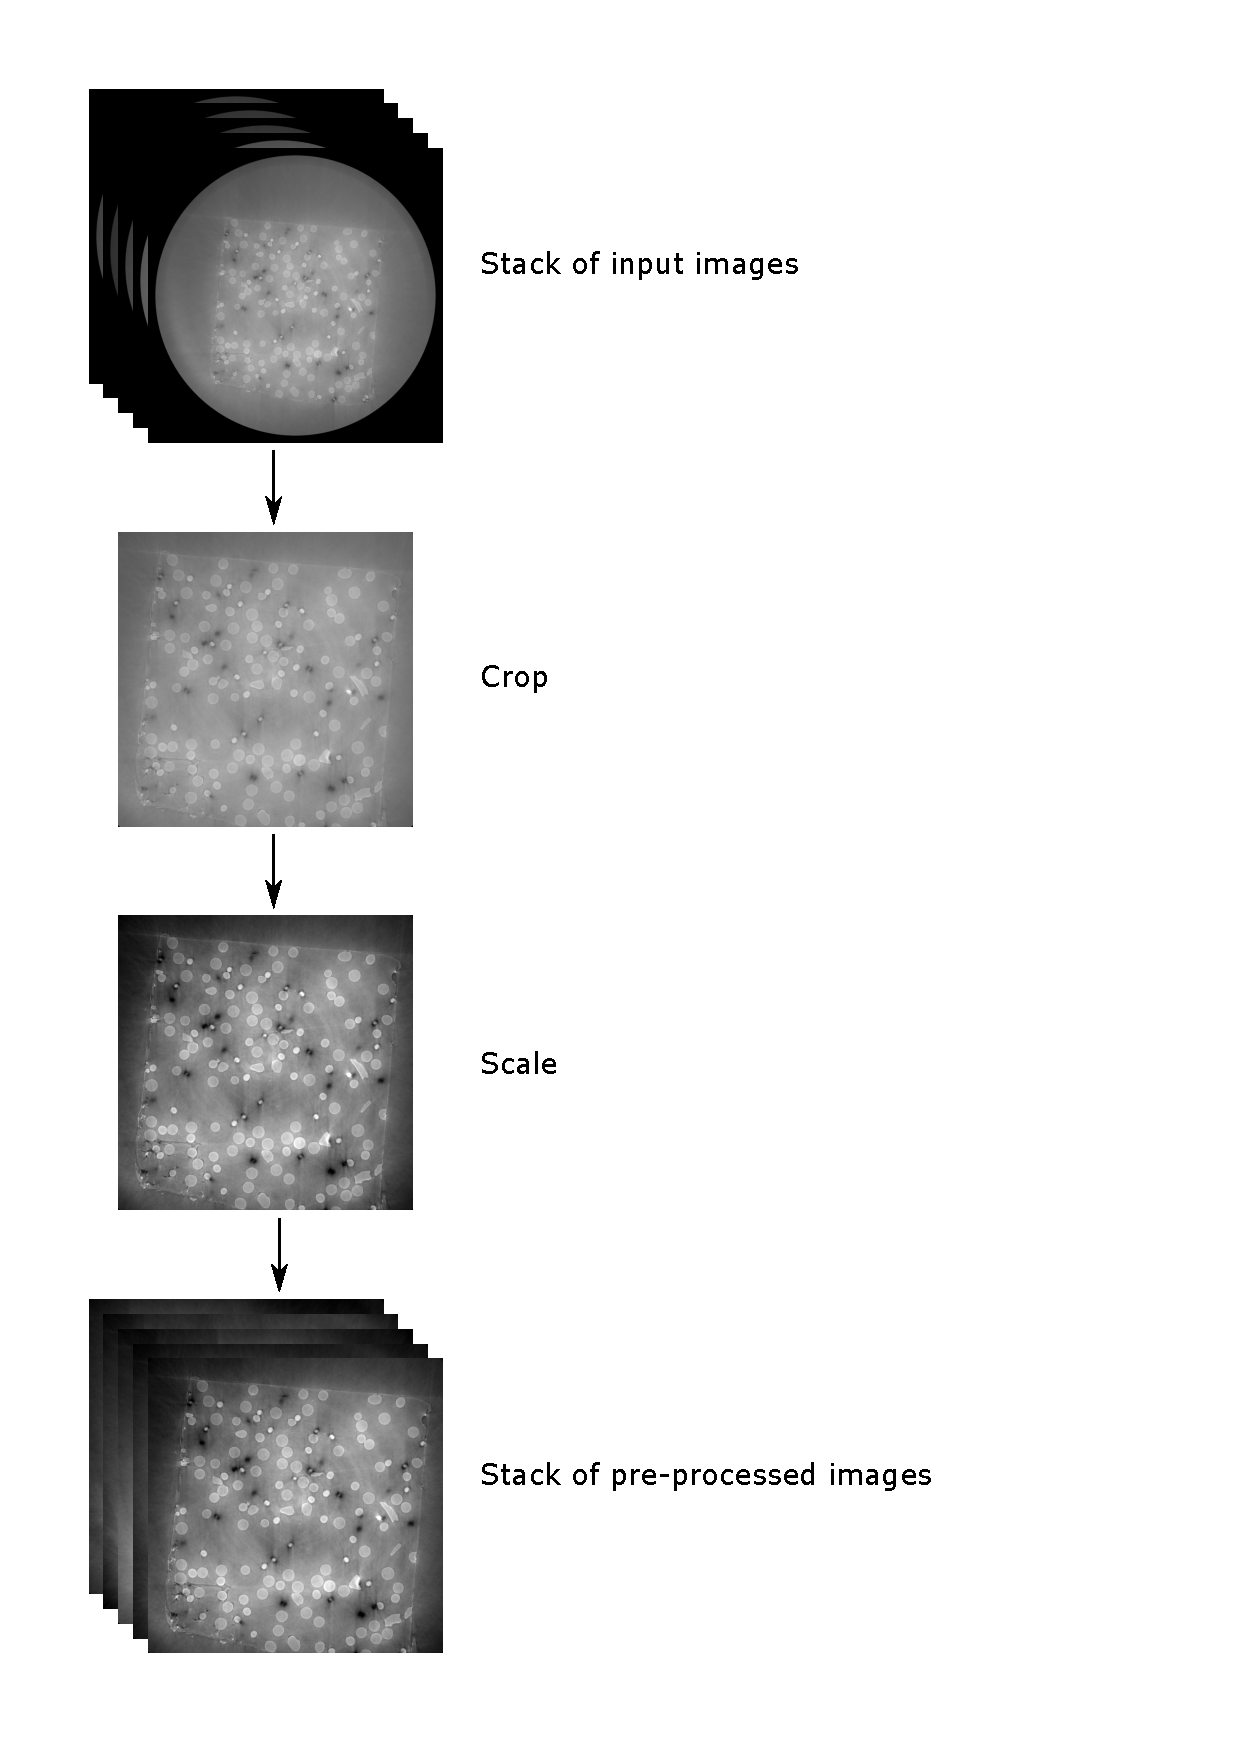
\includegraphics[width=.95\textwidth]{figures/compilingdatasetflowchart.pdf}
    \caption[Dataset creation flowchart]{Flowchart showing the process of compiling a dataset for training the TomoGAN denoising network. }
    \label{fig:compilingdatasetflowchart}
\end{figure}

\todo[inline]{Making a dataset: scaling, cropping, sorting, selecting only good images (e.g. ignore empty from top of stack). }